\subsection{Charakterystyka systemu czasu rzeczywistego}

\newtheorem{master_thesis}{Postawiony problem}[section]

\subsubsection{Opis samodzielnego systemu RT}

\par 
\tab Budowa ogólna systemów mikroprocesorowych w tym systemów czasu rzeczywistego lub architektur sensorycznych jest do siebie bardzo zbliżona. Każdy system posiada blok sensorów które dają sygnały wejściowe, blok mikrokontrolera/procesora lub innej jednostki decyzyjnej (np: FPGA lub innych programowalnych układów) oraz blok wyjściowy do którego trafia wynik przetworzonych sygnałów z bloku sensorycznego. \\
Poniżej zaprezentowano ogólny schemat systemu wbudowanego który z jednej strony poprzez sensory wejściowe odbiera sygnały z otaczającego go środowiska, z drugiej strony poprzez blok wyjściowy jest w stanie reagować na przychodzące sygnały np: poprzez fizyczną zmianę sygnału elektrycznego, sterownik silnika lub wysłanie określonej wiadomości poprzez podłączone medium komunikacyjne takie jak układ radiowy czy internet. \\

 \centerline{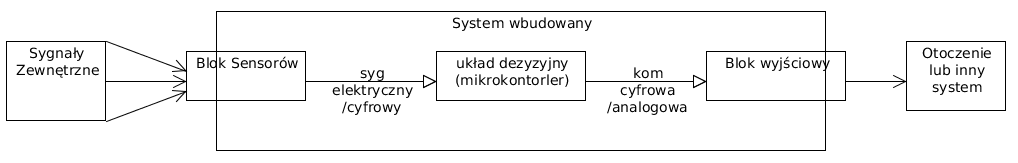
\includegraphics[scale=0.40]{./img/target_system/embedded_system_general.png}} 

\par
\tab
W przypadku systemów komunikujących się bezprzewodowo takich jak WSN blokiem wyjściowym oraz wejściowym jest układ radiowy służący do komunikacji z resztą systemu. Poniżej został przedstawiony schemat blokowy pojedyńczego węzła wchodzącego w skład bezprzewodowej sieci sensorycznej. \\

 \centerline{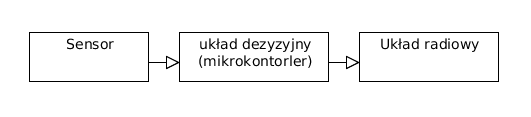
\includegraphics[scale=0.40]{./img/target_system/Uklad_badany.png}} 

\subsubsection{Przedstawienie badanego problemu}

\par 
\tab
Systemy czasu rzeczywistego w połączeniu z sieciami typu WSN wnoszą dodatkowy poziom skomplikowania ponieważ na szybkość odpowiedzi oprócz działania samego systemu operacyjnego wpływa również szybkość i niezawodność sieci w której odbywa się komunikacja między poszczególnymi węzłami. Jednakże takie połączenie wnosi bardzo wiele możliwości sprawiając że takie architektury mogą czerpać z największych zalet systemów RT oraz bezprzewodowych sieci sensorycznych. //
Przykładem takiego połączenia mogą być wszystkie interfejsy użytkownika wymagające odpowiedzi w czasie rzeczywistym takie jak np: bezprzewodowa kierownica, sterownik do urządzeń elektromedycznych, sterownik do zdalnie prowadzonych robotów i wiele innych zastosowań gdzie wyeliminowanie klasycznego połączenia kablowego wnosi wiele wygody, oszczędza miejsce czy daje możliwości lepszej pracy przy zachowaniu dotychczasowych cech czyli pewności działania, odpowiedzi w określonym czasie i bezpieczeństwa.

Celem niniejszej pracy jest zbadanie bezpieczeństwa systemu czasu rzeczywistego używającego do komunikacji sieci typu WSN na przykładzie bezprzewodowego włącznika do zastosowań medycznych. \\

\begin{master_thesis}
\textbf{ \textit{Analiza bezpieczeństwa bezprzewodowego włącznika nożnego do zastosowań  medycznych} }
\end{master_thesis}

Całość pracy obejmuje również elastyczną implementację takiego systemu w oparciu o różne systemy ogólno dostępne na rynku, która pozwoli na wnikliwą analizę wszystkich części składowych problemu.

Jako efekt pracy powstanie ocena przykładowej implementacji w ujęciu wymagań stawianych przez twarde systemy czasu rzeczywistego jakimi są niewątpliwie sterowniki urządzeń medycznych


\subsubsection{Opis domeny zagadnienia}

\par 
\tab Koncepcja wprowadzenia bezprzewodowych sterowników do urządzeń medycznych nie jest niczym nowym. Od czasu kiedy stały się popularne bezprzewodowe interfejsy użytkownika wszystkie branże zaczęły się zastanawiać czy w celu uzyskania dodatkowych profitów mogą wprowadzić bezprzewodowe interfejsy użytkownika, w zamian za istniejące kablowe/stykowe, do swojego biznesu. Dla zastosowań w których bezpieczeństwo i wysoka niezawodność transmisji nie jest krytyczną wytyczną rozwiązania te przyjęły się bardzo szybko, natomiast w branżach takich jak medycyna gdzie wytycznymi projektu rządzi bezpieczeństwo pacjenta i niezawodność urządzenia do tej pory najczęściej spotykanymi rozwiązaniami są połączenia za pomocą grubych kabli. \\

\tab Podczas mojej pierwszej pracy jako inżynier systemów wbudowanych w polskiej firmie prowadzącej sprzedaż urządzeń medycznych w tym laserów dużej mocy do zastosowań m.in. w chirurgii, pojawiła się koncepcja ułatwienia pracy chirurgom poprzez eliminacje rozmiarów urządzeń. Dla lekarzy problematyczne stały się ograniczenia wynikające z połączenia włącznika nożnego lasera za pomocą grubego kabla do głównego ciała urządzenia. Przewód elektryczny często był uszkadzany przez zgniatanie go innymi obiektami na sali zabiegowej, również połączenie przewodem utrudniało lekarzom komfort pracy ponieważ byli oni ograniczeni przewodem leżącym na podłodze przy stole zabiegowym który prowadził do lasera medycznego który często był niemobilnym urządzeniem przeznaczonym do umieszczenia w stałym miejscu. \\

\tab Ponieważ na pytanie czy wprowadzenie bezprzewodowego włącznika ułatwiłoby pracę i oczywiście skłoniło do zakupu, lekarze odpowiedzieli twierdząco firma postanowiła stworzyć takie rozwiązanie mimo tego że była to funkcjonalność rzadko spotykana na rynku dostępna tylko w niektórych urządzeniach. \\

Poniżej fotografia stosowanego przewodowego włącznika nożnego do zastosowań medycznych

 \centerline{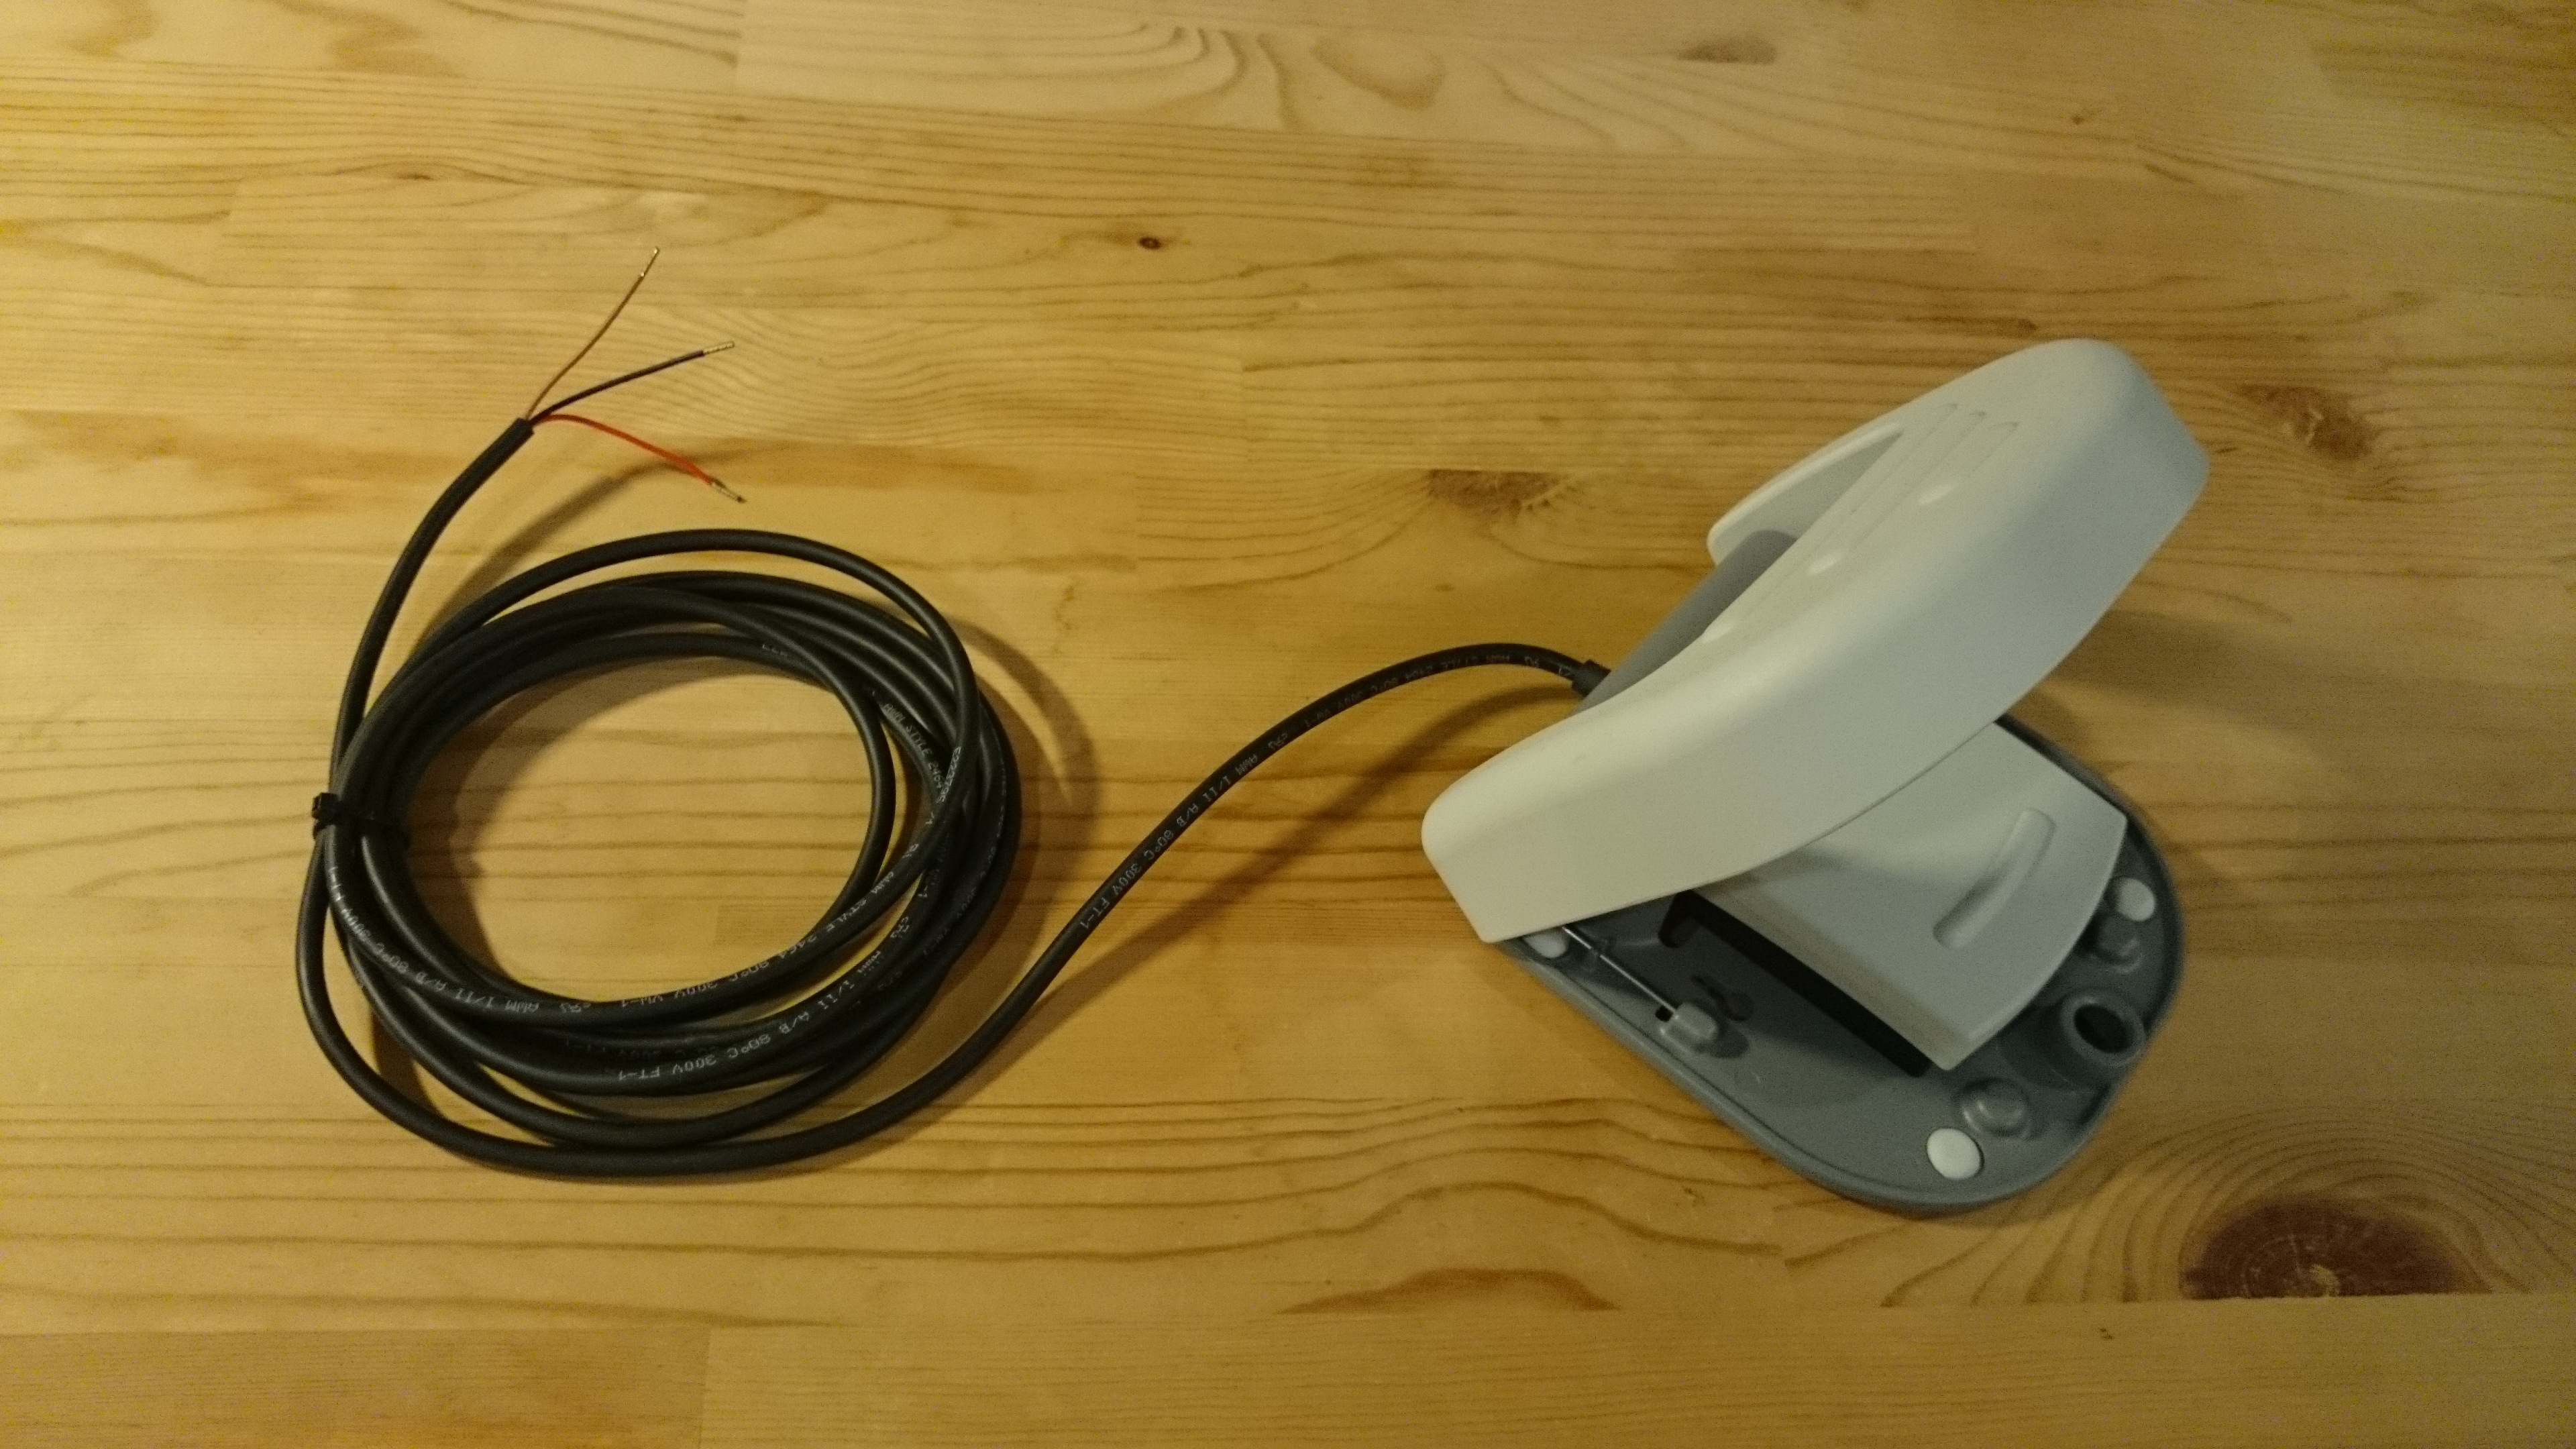
\includegraphics[scale=0.10]{./img/target_system/wlacznik_nozny.jpg}}

Oraz urządzenia lasera medycznego w tym przypadku jest to laser diodowy:

\centerline{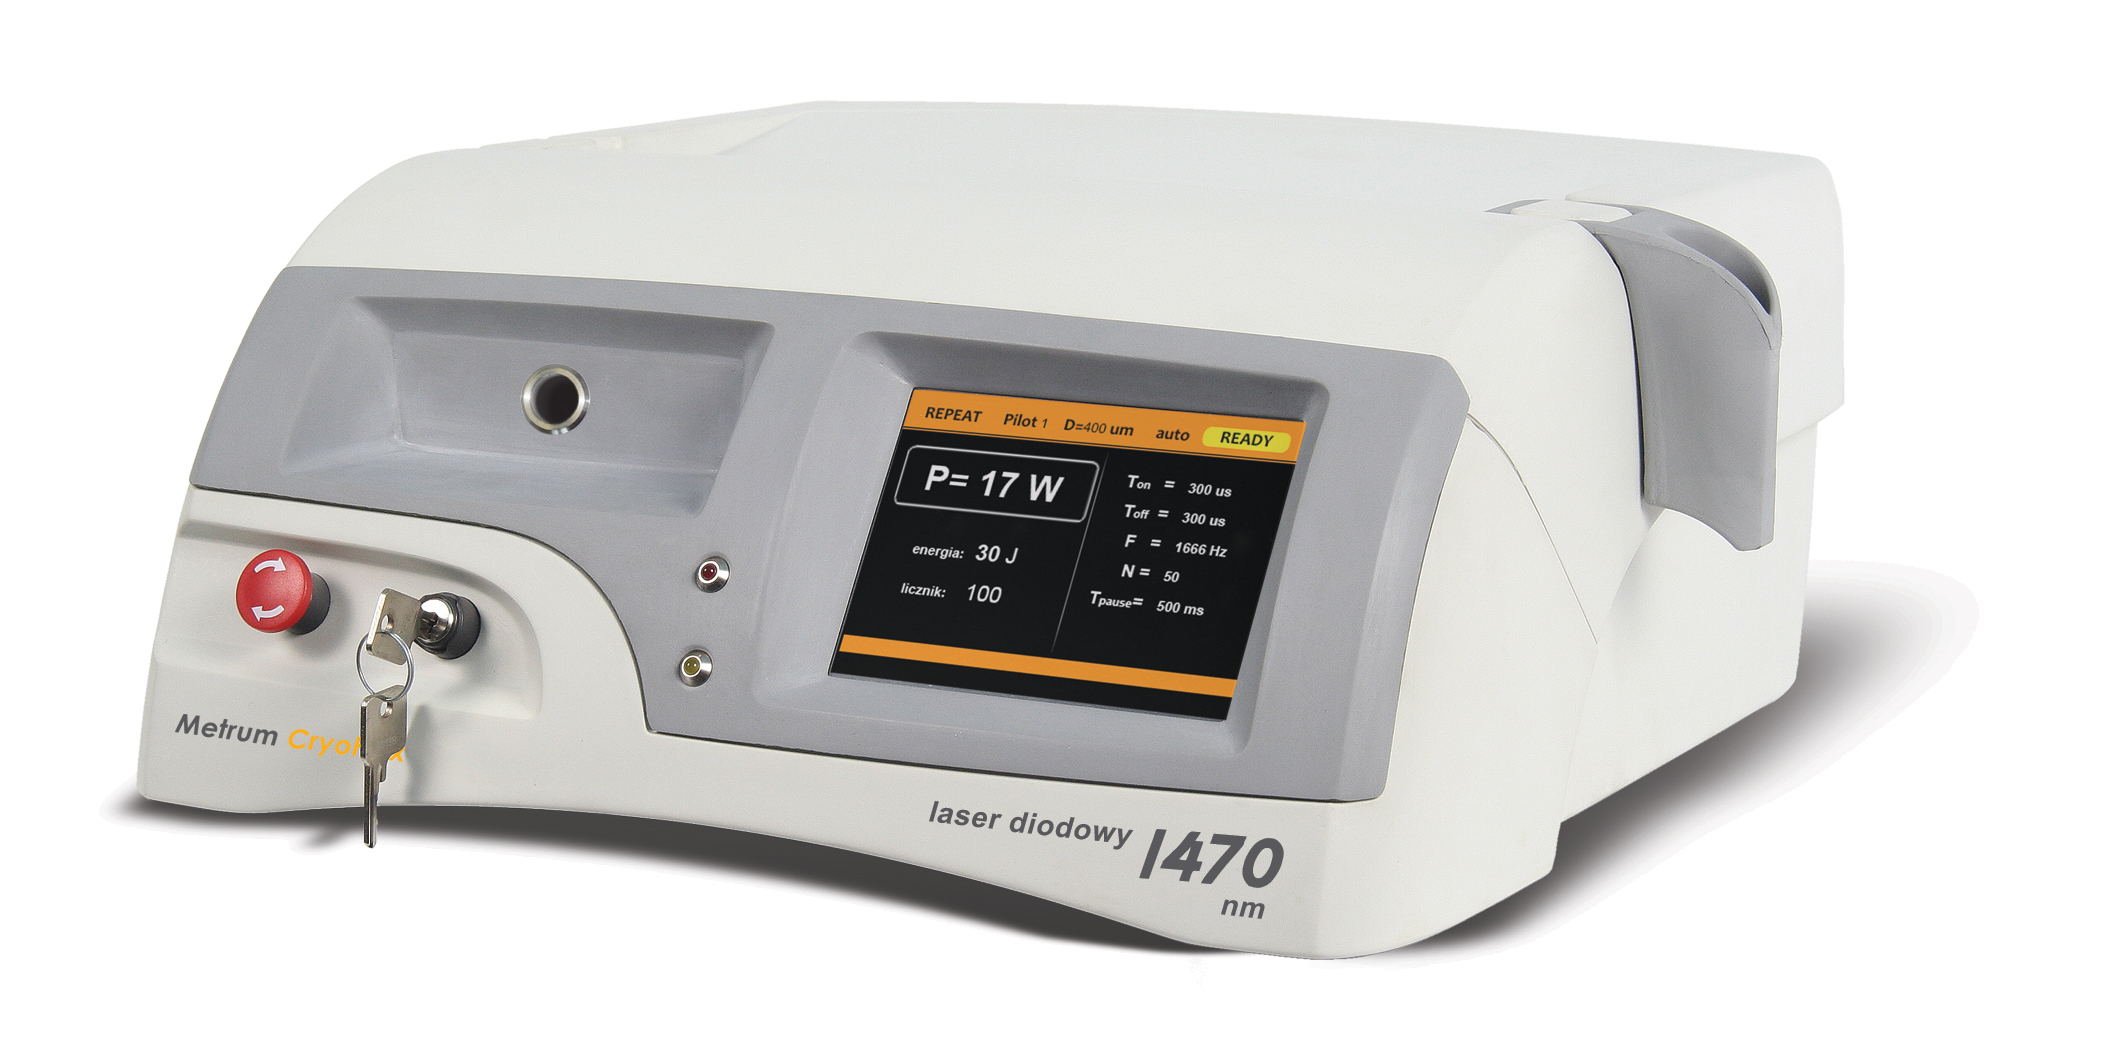
\includegraphics[scale=0.20]{./img/target_system/D1470_laser.jpg}} 

Jak widać laser jest dużym solidnym urządzeniem do którego od tyłu obudowy jest wczepiany włącznik za pomocą solidnego kabla o średnicy \diameter 6 mm. \\

\subsubsection{Analiza części składowych problemu} \mbox{}\\

Całość projektu systemu czasu rzeczywistego opartego o bezprzewodowe sieci sensoryczne można podzielić ogólnie na następujące częsci: \\

\begin{enumerate}
\item Ogólny projekt architektury systemu 
\item Wybór poszczególnych modułów systemu
\item Wyszczególnienie funkcjonalności czasu rzeczywistego
\item Stworzenie łańcucha procesu RT oraz zbadanie które moduły mają na niego wpływ
\item Przetestowanie łańcucha RT w zmiennych zewnętrznych warunkach 
\item Przetestowanie bezpieczeństwa systemu od zewnątrz i określenie potencjalnych niebezpieczeństw
\end{enumerate}

\paragraph{Ogólny projekt architektury systemu}\mbox{}\\
\tab W analizowanym przypadku system bezprzewodowego włącznika będzie składał się z dwóch węzłów: nadawczego który będzie zajmował się detekcją wł/wył oraz odbiorczego który będzie dawał sygnał do lasera medycznego o tym jaki jest obecnie stan włącznika.
Dla samego sterownika lasera jest niewidoczne skąd bierze się sygnał: czy z włącznika podłączanego kablem czy bezprzewodowego. Kontroler widzi jedynie zmieniający się stan wejściowy określający w jakim stanie jest włącznik.
\tab Oba węzły mają podobną budowę jak przykładowy węzeł z sekcji. -uklad badany

\centerline{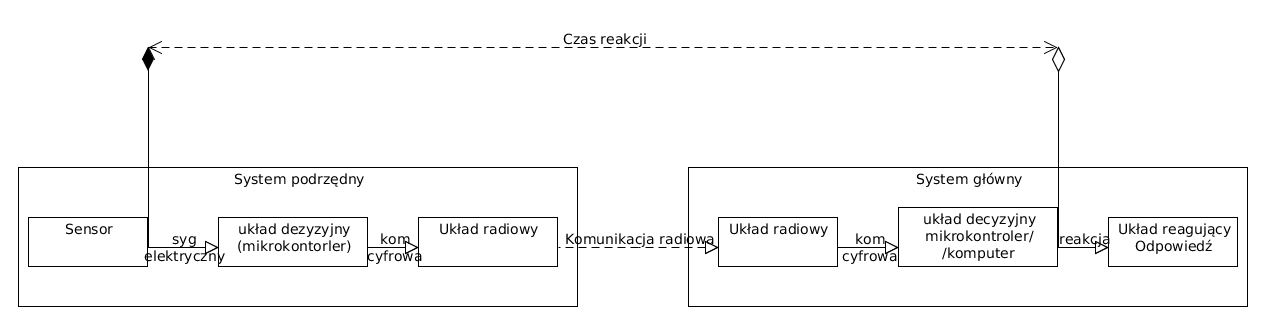
\includegraphics[scale=0.40]{./img/target_system/badany_system.png}} 

\paragraph{Wybór poszczególnych modułów systemu} \mbox{}\\
\tab W celu wyeliminowania z analizy elementów takich jak rózna implementacja standardów radiowych takich jak ZigBee lub BLE w projekcie zostanie użyty moduł typu OME czyli gotowy nadajnik z zaimplementowanymi warstwami protokołu radiowego.
Jako jednostka centralna zostanie użyty szybki mikrokontroler tak aby jego prędkość była pomijalna. Wybór padł na procesor ARM Cortex-M4 jako obecny standard przemysłowy dla systemów o średniej skali integracji.
System RT będzie również wybrany z pośród ogólnodostępnych standardów na rynku, ważną cechą przy tym wyborze jest otwartość kodu źródłowego oraz dobra dokumentacja.

\paragraph{Wyszczególnienie funkcjonalności czasu rzeczywistego} \mbox{}\\
\tab Każdy system elektroniczny posiada kilka standardowych funkcjonalności takich jak zarządzanie zasilaniem, przetwarzanie sygnałów przychodzących których źródłem mogą być dowolne czujniki dołączone do systemu.
Spośród wszystkich funkcjonalności często jako konstruktorzy systemu wyodrębniamy główne funkcjonalności, czyli najczęściej są to takie dla których de-facto tworzymy cały system. W Bezprzewodowych sieciach sensorycznych często spotykamy się z taką budową gdzie za jedną funkcjonalność odpowiada jeden węzeł sieci. \\
Przydładowo mając prostą sieć WSN do zastosowań w automatyce domowej dostarczamy klientowi następujące funkcjonalności: pomiar temperatur wewnątrz domu, na zewnątrz, sterowanie bramą wjazdową i włączaniem światła po zmroku gdy w pobliżu pojawi się mieszkaniec. Możemy śmiało spodziewać się 4 czujników które będą połączone radiowo i dodatkowo jakiejś jednostki głównej której funkcją jest zarządzanie siecią. O ile pomiar temperatury może nie wydawać się krytyczną kwestią o tyle sterowanie bramą wjazdową na posesję trzeba traktować jako funkcjonalność o najwyższym priorytecie ponieważ sytuacja w której zmęczony po całym dniu w pracy pan domu nie może otworzyć bramy wjazdowej pilotem i wjechać do domu bo właśnie następuje odczyt temperatury wydaje się być groteskowa. \\
Z tego powodu wszystkie funkcjonalności w systemie powinny być uporządkowane w pewnej hierarchii. 
W systemach czasu rzeczywistego główne funkcjonalności najczęściej są właśnie procesami czasu rzeczywistego, czyli takimi które muszą być obsłużone natychmiast po zaistnieniu nie zależnie od tego w jakim stanie obecnie znajduje się cały system.
Oprócz głównych funkcjonalności które czasem są nazywane mianem domenowych (czyli takich które decydują o branży w jakiej wykorzystywane jest całe urządzenie) występują jeszcze często nie zauważane przez użytkowników procesy o możliwym jeszcze wyższym priorytecie niż proces domenowy. \\
Przykładowo w naszym systemie czasu rzeczywistego bezprzewodowego włącznika nożnego stan włącznika (0-nie wciśnięty, 1-wciśnięty) musi być wiernie przeniesiony za pomocą drogi radiowej do ciała głównego lasera ponieważ ten sygnał będzie następnie odpowiadał stanowi włączenia wyłączenia Diody. Sam włącznik jest urządzeniem zasilanym bateryjnie z tego powodu warunkiem koniecznym do działania jest stan naładowania baterii, sytuacją nie dopuszczalną jest aby rozpocząć zabieg z baterią będącą na pograniczu wyczerpania ponieważ w tym momencie zachowanie całego włącznika mogłoby być nieprzewidywalne a więc również stan diody laserowej mógłby być nieprzewidywalny a sytuacja taka jest wysoce niedopuszczalna.
Kolejnym bardzo ważnym elementem całego systemu jest autoryzacja włącznika, czyli sprawdzenie czy włącznik komunikujący się z laserem jest dedykowany do tego lasera a więc tylko jeden włącznik może sterować jednym laserem i musi być to z góry określone.
Oprócz zastosowania mającego na celu zapobieganie \textit{Hakowania} systemu które nie mniej jest bardzo ważne, możemy sobie wyobrazić sytuację gdzie w dwóch gabinetach obok siebie pracują dwa lasery medyczne z bezprzewodowymi włącznikami. Aby system był bezpieczny te włączniki nie mogą na siebie oddziaływać. \\
 \centerline{W systemach RT Funkcjonalności możemy podzielić ze względu na: } \\
	\begin{itemize}
    	\item Krytyczność ze względu na czas
        \item Krytyczność ze względu na pełnioną funkcję
    \end{itemize}
    
Hierarchię między procesami określa się na początku tworzenia systemu na podstawie wymagań domenowych oraz technicznych. W naszym przypadku wszystkie funkcjonalności podzielimy na 3 grupy: Najwyższy priorytet, Wysoki priorytet oraz Niski priorytet. \\

   \centerline{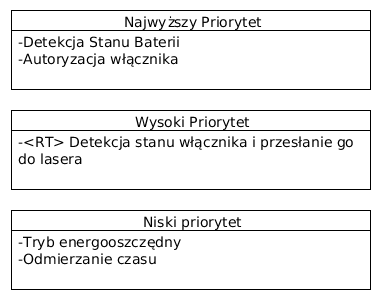
\includegraphics[scale=0.60]{./img/target_system/hierarchiaProcesow.png}} 


\paragraph{Stworzenie łańcucha procesu RT oraz zbadanie które moduły mają na niego wpływ} \mbox{}\\

\tab Głównym obiektem badań niniejszej pracy jest proces RT mający na celu przeniesienie stanu włącznika nożnego za pomocą fal radiowych na wejście lasera, która to włącza, wyłącza wiązkę lasera.
Jako argument wejściowy przyjmuje stan włącznika (wartość logiczna 0-1) a jako wynik zwraca również wartość logiczną. 
Matematycznie opisując przyjmujemy że x to stan włącznika a F(x) jest stanem przeniesionym bezpośrednio do ciała lasera: \\

\centerline{ $ F(x) = x  $ }

\centerline{  gdzie $  x, F(x) \in {-1,1} $ }

Na pierwszy rzut oka widać że funkcja jest trywialna i jedyne co robi to przenosi stan wejścia na wyjście jednak trzeba pamiętać że taki prosty model matematyczny nie uwzględnia opóźnienia które występuje w układzie i które badamy.
Następnie znając jakie są zależności wyjścia (F) od wejścia (x) należy rozbić na jednostkowe składowe przebieg całego procesu aby móc przeanalizować które elementy łańcucha wprowadzają opóźnienie i jakiego rodzaju jest to opóźnienie. \\
Poniżej znajduje się kompletny łańcuch z wyodrębnionymi elementami składowymi.\\

   \centerline{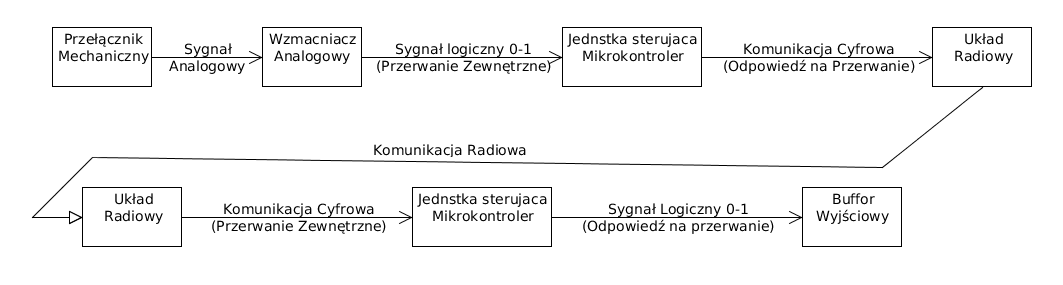
\includegraphics[scale=0.50]{./img/target_system/Lancuch_RT.png}} 

Idąc od lewej strony cały proces zaczyna się od przełącznika mechanicznego który w tym przypadku jest źródłem sygnału. Możemy sobie założyć że stan tego przełącznika określa dla nas czas zerowy czyli moment w którym cały proces się zaczyna z tego powodu taki przełącznik nie będzie wliczany do źródeł opóźnienia.\\
Następny element łańcucha czasu rzeczywistego to wzmacniacz analogowy. Ponieważ styki mechaniczne w momencie zwierania przez krótki ułamek czasu wprowadzają stan nieustalony pełen zakłóceń i drgań aby dokładnie wiedzieć w którym momencie nastąpiło fizyczne zetknięcie metali stosuje się filtry dolno przepustowe oraz wzmacniacz sygnału, ponieważ te dwie funkcjonalności można zrealizować za pomocą wzmacniacza operacyjnego przyjmujemy że jest to pojedyńczy blok. Ponieważ odpowiedź wzmacniacza operacyjnego w układzie filtru dolnoprzepustowego wyraża się w mikrosekundach możemy sobie przyjąć że ten blok ma pomijalnie mały stały czas który możemy zignorować (bardzo często w systemach czasu rzeczywistego pomijamy elementy elektroniczne analogowe ponieważ są one dużo szybsze od cyfrowych a ich czas jest stały) \\
Trzeci element łańcucha to mikrokontroler. W naszym przypadku uC działa pod wpływem tzw. RTOS (Real Time Operating System). Systemy takie mają tą zależność że ustawia się dla nich okres działania zegara systemowego (tzw. sys tick) który determinuje czas w jakim jest przewidywana zmiana wykonywania obecnego programu i obsługa funkcjonalności czasu rzeczywistego. Tutaj zostanie użyty standardowy czas dla tego typu systemów wynoszący 1ms, dzięki temu zyskujemy pewność, że maxymalnie w przeciągu 1ms od nastąpienia przerwania zewnętrznego zostanie uruchomiony kod który obsłuży to przerwanie. Z tego powodu dla mikrokontrolera należy przyjąć największe możliwe opóźnienie które wyniesie 1ms plus czas transmisji cyfrowej w celu nadania wiadomości radiowej do nadajnika.\\
Czwartym blokiem jest blok nadajnika radiowego, tutaj czas działania modułu jest zależny od wykonania przez producenta.
Blok ten łączy się z blokiem odbiorczym poprzez transmisję drogą radiową, dla ułatwienia w pierwszym podejściu możemy sobie przyjąć że będziemy traktować czas pomiędzy zleceniem transmisji wiadomości drogą radiową z jednego modułu RF do drugiego jako jeden czas, i jeśli będzie taka potrzeba to tenczas będziemy dalej rozbijać. \\
Przedostatni blok to mikrokontroler odbiorczy przyczepiony do ciała lasera tutaj mamy sytuację analogiczną jak w pierwszym uC.\\
Ostatni element łańcucha to bufor wyjściowy jest on analogiczny do wzmacniacza wejściowego, z tego powodu jego czas również możemy pominąć. \\
Podsumowując na całkowite opóżnienie składają się: \\

$ T_{calk} = T_{uC1} + T_{RFtransmit} + T_{uC2} $

$
 gdzie: \\
T_{uC1} \text{ : opóźnienie na wejściowym mikrokontrolerze} \\
T_{RFtransmit}  \text{ : opóźnienie podczas transmisji RF między nadajnikami} \\
T_{uC2} \text{ : opóźnienie na wyjściowym mikrokontrolerze } \\
$
\mbox{}\\

Dodatkowo czas transmisji radiowej możemy również rozbić na: \\

$ T_{RFtransmit} = T_{transmiterDelay} + T_{air} + T_{reciverDelay} $

$
gdzie: \\
T_{air} \text{ : rzeczywisty czas transmisji radiowej } \\
T_{transmiterDelay}  \text{ : opóźnienie na transmiterze } \\
T_{reciverDelay} \text{ : opóźnienie na odbiorniku } \\
$
\mbox{}\\

\paragraph{Przetestowanie łańcucha RT w zmiennych zewnętrznych warunkach } \mbox{}\\

W celu sprawdzenia czy zaprojektowany system posiada deterministyczną odpowiedź w czasie należy wykonać oczywiście odpowiednie testy polegające na mierzeniu czasu odpowiedzi na przychodzące zdarzenie w czasie. W naszym wypadku będziemy mierzyć czas od momentu pojawienia się sygnału odpowiadającemu wciśnięciu włącznika do momentu pojawienia się odpowiadającego mu sygału na wejściu lasera. \\
Ponieważ w obecnej postaci system jest modularny i umożliwia prostą zamianę jego modułów na inne zostaną przetestowane dwa standardowe protokoły radiowe wykorzystywane w sieciach typu WSN a mianowicie:
oparty o standard 802.15.4 protokół ZigBee oraz implementujący standard 802.15.1 Bluetooth Low Energy. \\
Czyli całe testy zostaną podzielone na dwie grupy:
\begin{itemize}
    	\item Testy sieci typu WSN opartej o ZigBee
        \item Testy sieci typu WSN opartej o Bluetooth Low Energy
    \end{itemize}
Dodatkowo testy będą się odbywać w otoczeniu innych nadajników nadających na tych samych częstotliowściach i kanale oraz dodatkowo w otoczeniu sieci Wifi która jest obecnie wszechobecnie występującą emisją elektromagnetyczną. \\
Testy opóźnień zostaną wykonane za pomocą oscyloskopa cyfrowego firmy ATTEN o prędkości próbkowania 50MHz i rozdzielczości 500MSa/s. Dla potrzeb testów przyjmiemy sobie jako podstawową jednostkę odniesienia pomiarów czasu 1ms z powodu standardu narzuconego przez system czasu rzeczywistego działający na mikrokontrolerze, oraz z uwagi na standardy transmisji cyfrowej których prędkość transmisji podawana jest w kB/s (1000 Bitów na sekundę) czyli w odniesieniu do mili sekundy. \\

\paragraph{Przetestowanie bezpieczeństwa systemu od zewnątrz i określenie potencjalnych niebezpieczeństw} \mbox{}\\

Oprócz głównej funkcjonalności jaką zapewnia system włącznika nożnego, system musi również spełniać inne wymogi wobec wymienionych wcześniej funkcjonalności o najwyższym priorytecie czyli: prawidłowej autoryzacji między urządzeniem lasera a włącznikiem, zarządzanie zasilaniem przez włącznik czy odporność na zakłócenia. \\
Testy systemu oprócz pomiaru samego czasu reakcji na zmieniony stan włącznika nożnego będą również obejmować: 
\begin{itemize}
    	\item Omówienie bezpieczeństwa sieci ZigBee/BLE oraz przedstawienie najnowszych badań dotyczących bezpieczeństwa sieci dla których będzie testowany system i odniesienie ich do zaprojektowanego systemu.
        \item Prównanie zużycia energi podczas transmisji samych modułów radiowych
        \item Wpływ zakłóceń na sieci WSN oparte o ZigBee/BLE, tutaj z wyszczególnieniem, że ten wpływ będzie jedynie omówiony ponieważ zbadanie samego wpływu eksperymentalnie wymaga specjalistycznego sprzętu oraz warunków laboratoryjnych.
    \end{itemize}

\subsubsection{Proponowane rozwiązanie}

\tab Nawiązując do schematu blokowego sieci WSN w punkcie poświęconemu ogólnemu projektowi architektury systemu omówimy poszczególne moduły systemu oraz ich implementację.\\

\paragraph{Wybór wzmacniacza}

Jako pierwszy omówimy blok wzmacniacza. Funkcją jaką ma on pełnić jest filtrowanie i wzmacnianie sygnału pochodzącego z mechanicznego przełącznika. Istnieje kilka rozwiązań spotykanych w przemyśle które odpowiedzialność za tę funkcjonalność przenoszą na mikrokontroler poprzez implementacje filtru cyfrowego lub poprostu przez tzw debouncing czyli w momencie wykrycia zmiany wprowadzenia sztucznego opóźnienia w celu ustalenia stanu wejścia i ponownym pomiarze. W systemach ukierunkowanych na czas oraz niezawodność staramy się przeprowadzać możliwie jak najwięcej obróbki sygnału w postaci analogowej, ponieważ czas jest nieporównywalnie krótszy a samo rozwiązanie dużo bardziej niezawodne. \\
Przy tworzeniu takiego filtra analogowego należy określić jego charakterystykę a najbardziej skupić się na paśmie które chcemy filtrować oraz wzmocnieniu. W naszym przypadku chcemy filtrować wszystkie szybkie sygnały głównie takie jak drganie styków oraz zakłócenia elektromagnetyczne. Interesuje nas wolnozmienny sygnał który powstaje w momencie zwarcia przełącznika mechanicznego.
W tym celu możemy sobie spokojnie przyjąć że chcemy ucinać wszystkie sygnały o wyższej częstotliwości niż 25Hz (punkt ten nazywany jest passband-frequency) dzięki takiemu pasmu wyeliminujemy również szkodliwy wpływ promieniowania sieci energetycznej 50Hz (lub 40Hz w innych częściach świata). \\ 
Drugim parametrem jest wzmocnienie dzięki któremu będziemy w stanie "uwidocznić" przychodzący sygnał.W naszym wypadku możemy to wzmocnienie ustalić wartość z przedziału 1-10 który jest standardowy w tego typu mechanicznych układach i ma na celu zniwelowanie niedoskonałości elementów oraz szkodliwy wpływ ewentualnych zanieczyszczeń. My wybierzemy wzmocnienie równe 5.
Mając już parametry filtra należy określić matematyczną charakterystykę, wybór ten polega na doborze istniejącego modelu na podstawie charakterystyki widmowej. Poniżej znajduje się kilka standardowych charakterystyk widmowych dla filtrów dolno-przepustowych o zadanych parametrach

\centerline{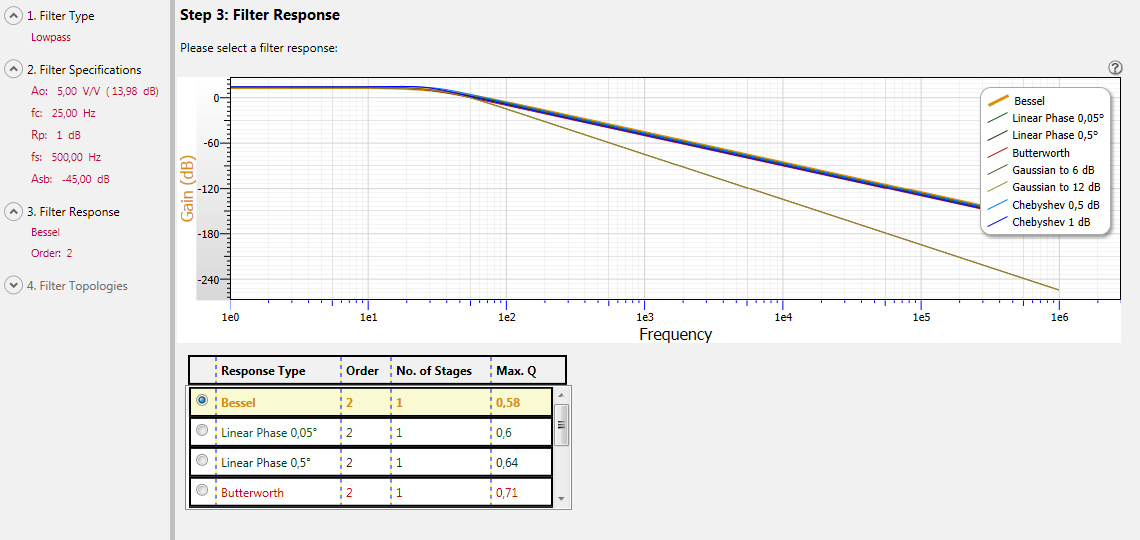
\includegraphics[scale=0.40]{./img/target_system/filtr/wybor_chrt_filtra.png}} 

Wyraźnie filtr bessla w tym porównaniu najlepiej wypada ponieważ jest on bardzo efektywny dla wolniejszych sygnałów. Tutaj także skorzystamy z niego. \\
Ważnym parametrem jest również stopień filtra, określa on zaz pomocą ilu fizycznych wzmacniaczy operacyjnych jesteśmy w stanie zbudować taki filtr, z tego powodu jeśli nie ma jakiś bardzo specjalistycznych wymagań należy wybrać charakterystykę o jak najmniejszej liczbie stopni. \\

Przykładowa budowa wzmacniacza operacyjnego dolno-przepustowego 2-giego stopnia w topologii Sallen-Key (standard w połączeniu elementów) wraz z charakterystykami fazowymi wzmocnienia oraz przesunięcia fazowego.

\centerline{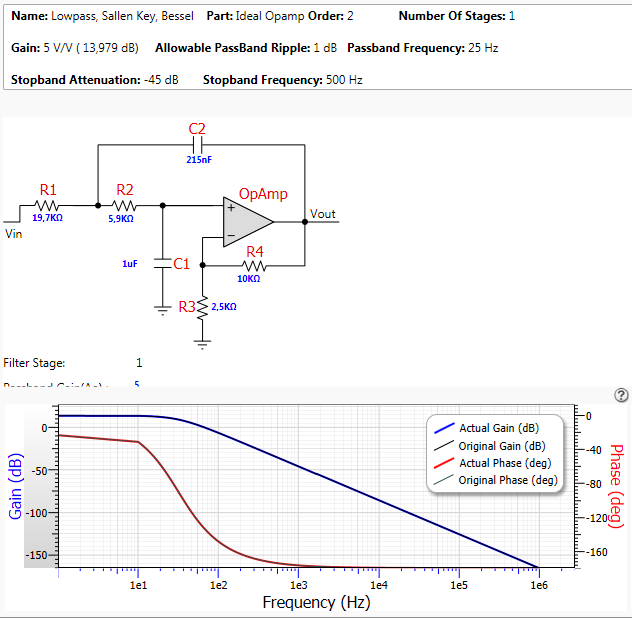
\includegraphics[scale=0.40]{./img/target_system/filtr/filter_design.png}} 

\paragraph{Wybór układu mikroprocesorowego i systemu RT}

Kolejnym elementem łańcucha czasu rzeczywistego jest układ mikrokontrolera. Obecnie panującym standardem na rynku mikrokontrolerów są układy zawierające rdzenie o architekturze ARM-Cortex. W naszym przypadku również skorzystamy z takiego układu ponieważ jest on ogólnodostępny w sprzedaży i istnieje wiele narzędzi wspierających pracę z takimi układami. Jako konkretny model wybór padł na układ firmy NXP LPC4330, należy on do rodziny mikrokontrolerów Cortex-M4 czyli najbardziej zaawansowanych układów z rodziny Medium Performance. Sam procesor LPC4330 ma możliwość działania na częstotliwości ponad 200MHz i jest on w momencie pisania tej pracy najszybszym ogólnodostępnym mikrokontrolerem w sprzedaży. \\
Wybór najszybszego mikrokontrolera pozwoli na zmniejszenie znaczenia prędkości wykonywania programu na mikrokontrolerze oraz kwestii technicznych związanych z budową samego układu peryferiów mikrokontrolera. Często konstruktorzy przypisują zbyt duże znaczenie do samej prędkości wykonywanego kodu podczas gdy największe opóźnienie rodzą się z powodu powolności transmisji, opóźnień związanych z odczytami z zewnętrznych układów. Do celów projektu zostanie użyta platforma ewaluacyjna dla mikrokontrolerów LPC4330 o nazwie \textit{"LPC4330-Xplorer"}
Na płytce ewaluacyjnej LPC4330-Xplorer oprócz micro-controllera znajduje się wiele ciekawych peryferiów takich jak przetworniki ADC do zastosowań audio, karta pamięci micro-sd, gniazdo i moduł ETH oraz porty we/wy w których skład wchodzi ponad 50 pinów GPIO pozwalających na podpięcie do modułu dowolnych peryferiów. Do portów tych zostanie podłączony wzmacniacz operacyjny oraz moduły radiowe służące do komunikacji między węzłami sieci. Płytka również posiada kryształ kwarcowy o dokładności +/-20ppm umożliwiający bardzo wysoką dokładność zegaru traktującego mikrokontroler.\\

\centerline{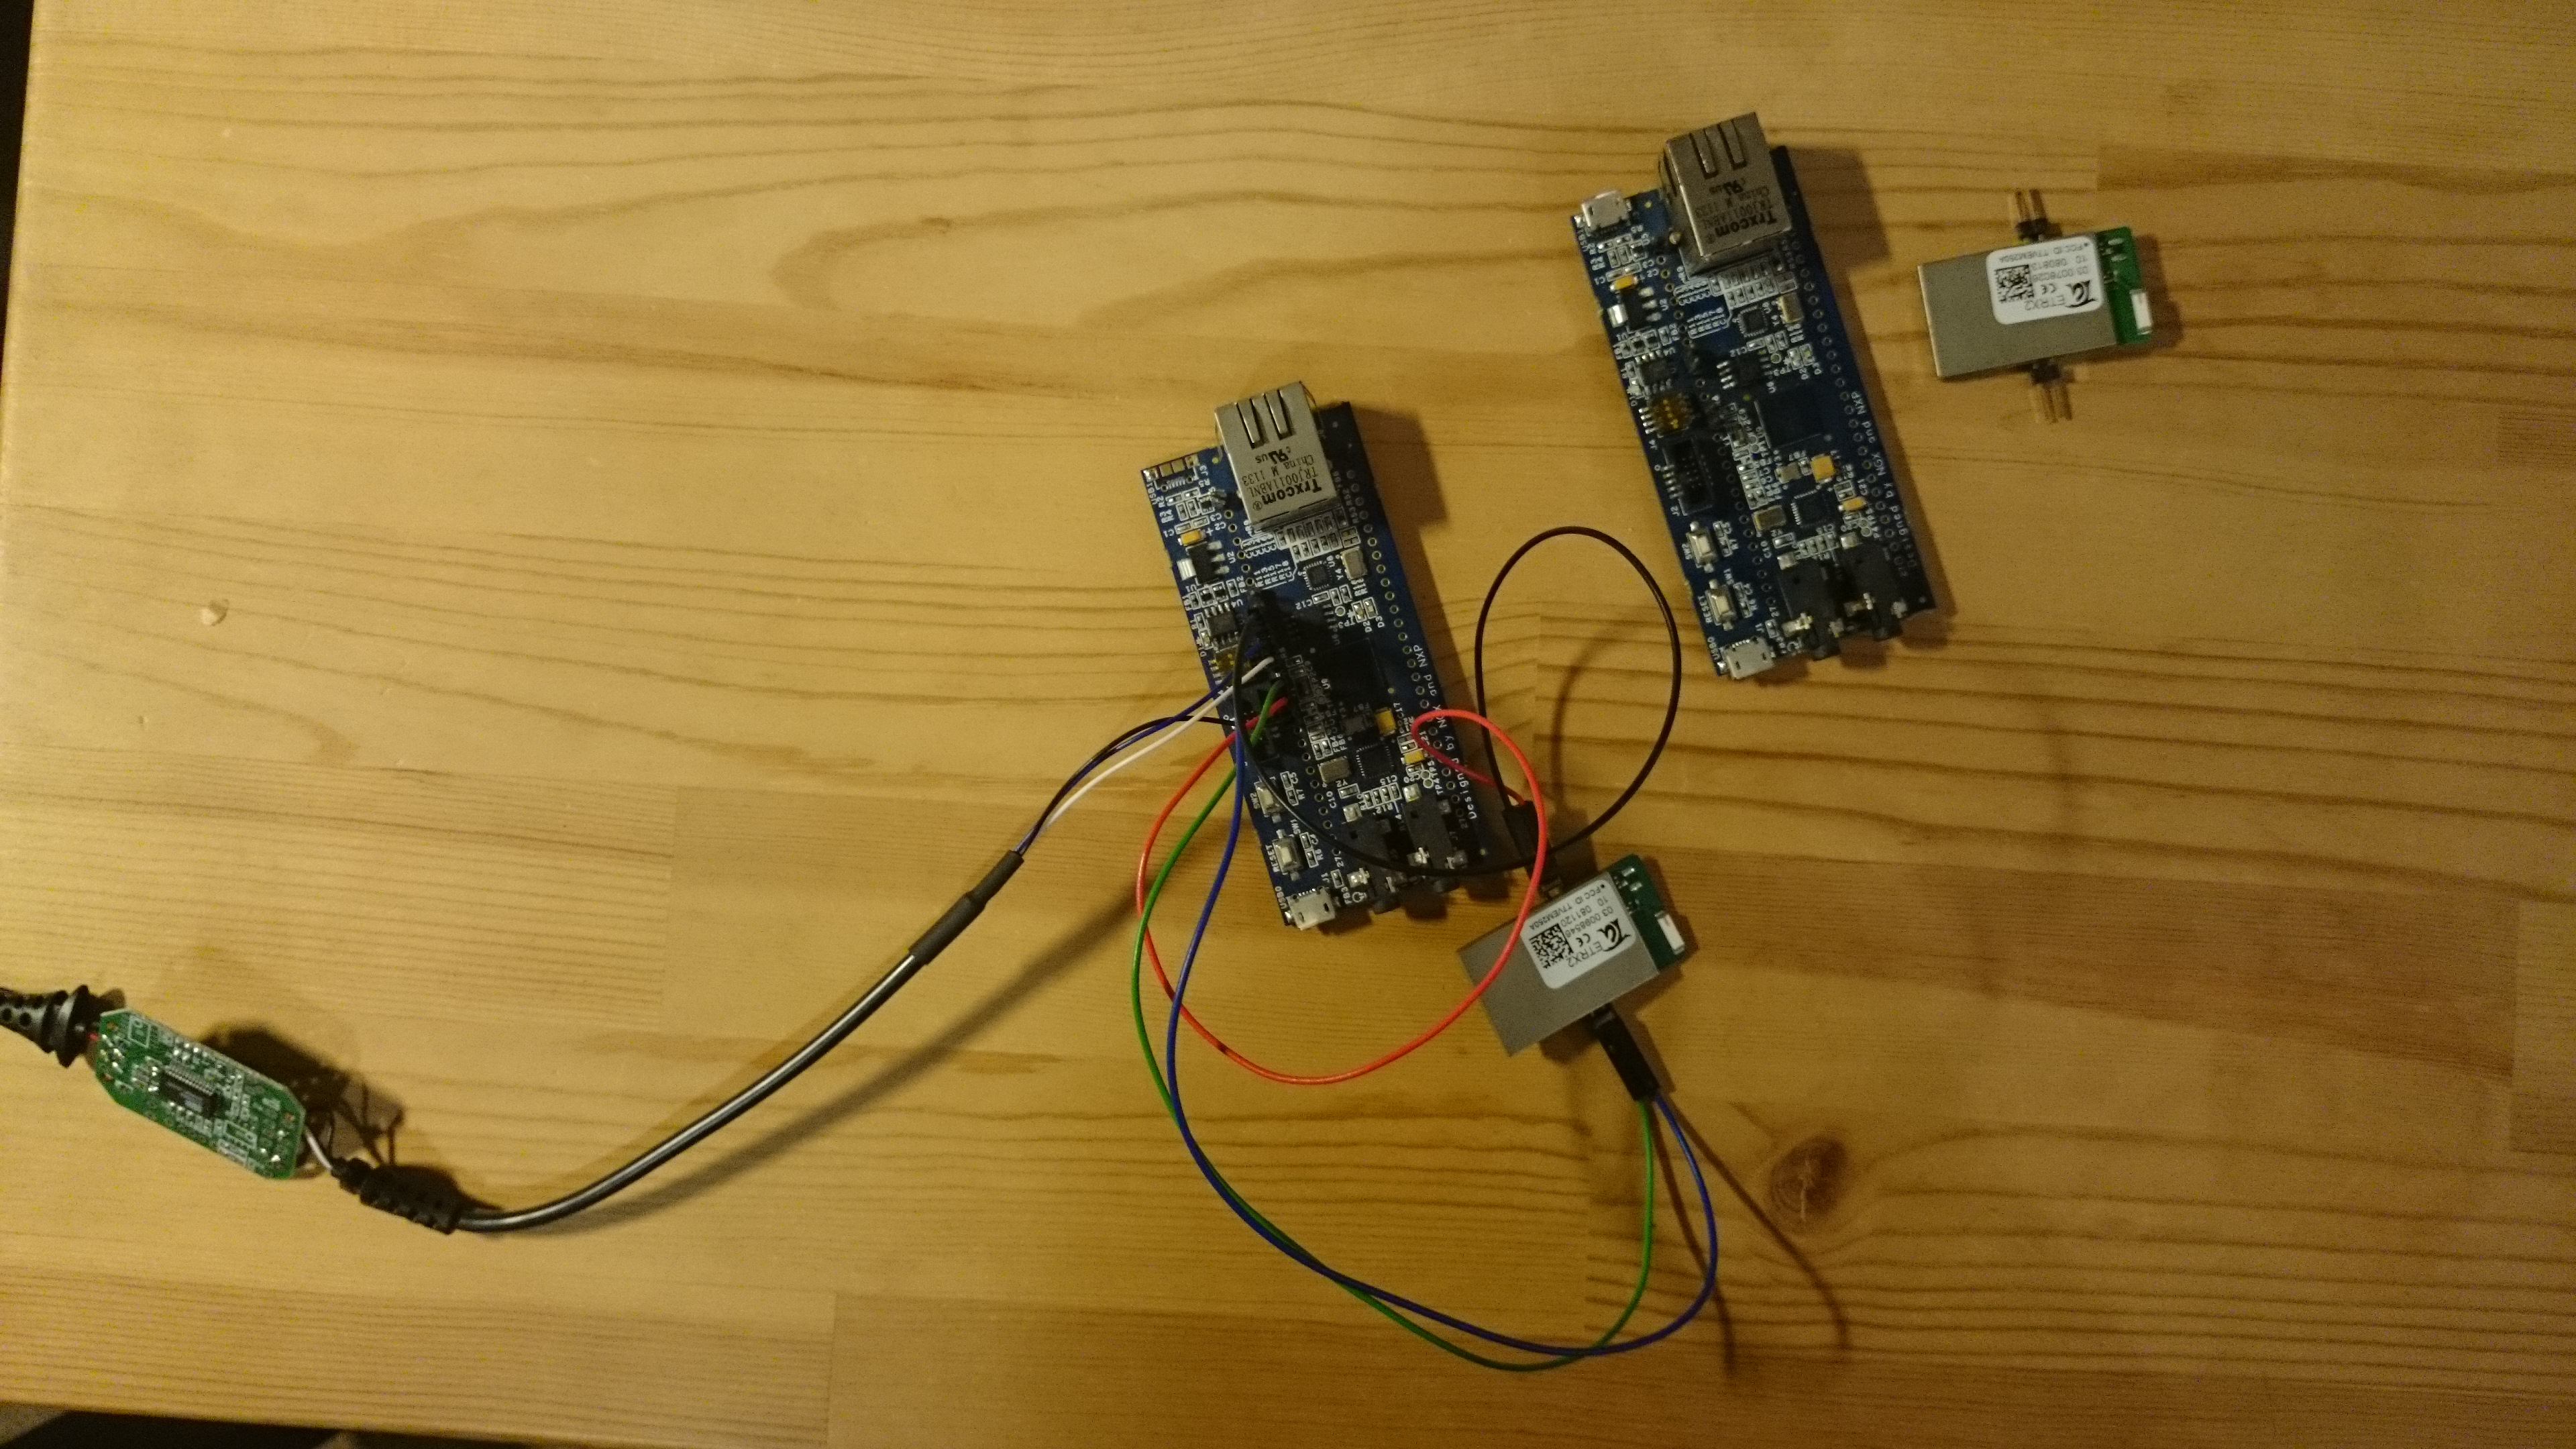
\includegraphics[scale=0.10]{./img/target_system/lpc4330-xplorer.jpg}} 

Do mikrokontrolera trzeba również dobrać odpowiedni system czasu rzeczywistego. W najprostrzym przypadku można stworzyć zwykły sekwencyjny program oparty o pętle główną (tzn. single-loop system), natomiast do bardziej skomplikowanych zastosowań często bezpieczniej jest użyć gotowego systemu. Na rynku istnieje wiele komercyjnych i otwartych RTOS-ów. W naszym przypadku posłużymy się otwartym systemem czasu rzeczywistego jakim jest projekt \textit{FreeRTOS}. \\
FreeRTOS jest systemem czasu rzeczywistego dostarczającym wszystkie najważniejsze funkcjonalności takie jak obsługa przerwań, planista, mechanizm kolejkowania czy priorytetyzacji zadań oraz również precyzyjne odliczanie czasu bez względu na obciążenie systemu.
Jest on również często używany jako standard rynkowy, ponieważ projekt jest otwarty i korzysta z niego wielu programistów na całym świecie. \\

\paragraph{Dobór układów transmisji radiowej}

Jak zostało wspomniane wcześniej, w ramach niniejszej pracy będziemy rozważać dwa typy transmisji radiowej opratej o standard ZigBee oraz BLE. Aby zrealizować taką transmisję należy skorzystać z odpowiednich układów radiowych oraz anteny. W naszym przypadku nie będziemy tworzyć od zera takiego modułu na podstawie gotowych układów, ale użyjemy już gotowych w pełni autonomicznych układów dostępnych na rynku. Podejście takie zwalnia nas z odpowiedzialności za samą implementację protokołu transmisyjnego oraz daje w zamian przyzwoitą prędkość transmisji ponieważ producenci takich układów często są specjalistami w dziedzinie technologii której dotyczą moduły możemy z powodzeniem przyjąć że prędkość komunikacji za pomocą modułu będzie wymierna ze zdefiniowanymi przez protokół standardami. \\
I tak jako układ komunikacyjny ZigBee zostaną użyte moduły ETRX3 firmy telegesis:

\centerline{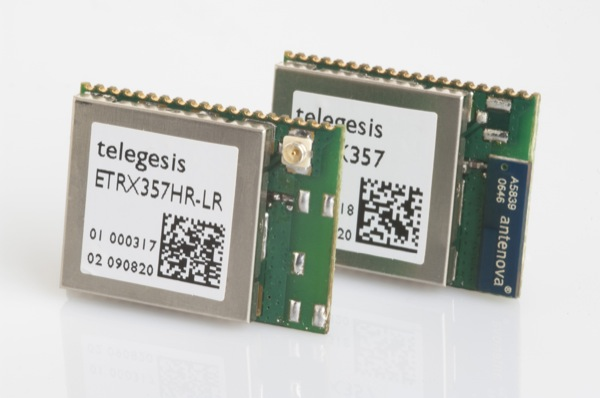
\includegraphics[scale=0.90]{./img/target_system/etrx3-modul.jpg}} 

Natomiast dla sieci Bluetooth smart moduł BLE112 firmy Bluegiga:

\centerline{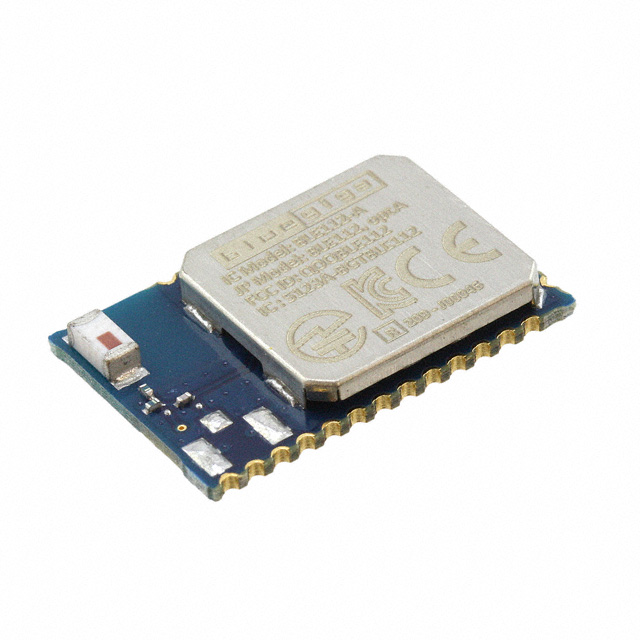
\includegraphics[scale=0.20]{./img/target_system/BLE112-module.jpg}} 

Obie firmy są liderami na rynku w zakresie komunikacji radiowej dlatego możemy sobie z pewnością założyć że wyniki osiągnięte przez ich moduły będą jak najbardziej adekwatne do implementowanych standardów.

\clearpage
